\section{Benchmark construction}
\label{sec:benchmark}

\textbf{Certified labels.} Each structure's crystal system, Bravais lattice, point group and space group
are derived from its coordinates by $\spg$ at the canonical tolerance, with a tolerance sweep that
quarantines any structure whose space group is not stable across it. On the kept set, label agreement with
the source databases is $220/220$ (one-sided exact 95\% lower bound $0.9865$).

\textbf{Composition exclusion.} No chemical composition in any evaluation set appears in training. Without
this, symmetry is partly predictable from composition alone, a published task \citep{cryspnet2003}, and a
model could score well without reading the image.

\textbf{A label ladder gives a difficulty axis.} Figure~\ref{fig:ladder} (right) scores four labels of
increasing granularity for the model-free arms. The oracle is flat across granularity because a
reconstruction is either right or wrong and all four labels follow from it; the cell-metric baseline falls
from 0.8952 at crystal system to 0.6810 at space group, because point group and space group depend on atom
positions that lattice parameters do not encode. The identifiability claim is therefore not specific to the
seven-way label.

\begin{figure}[t]
\centering
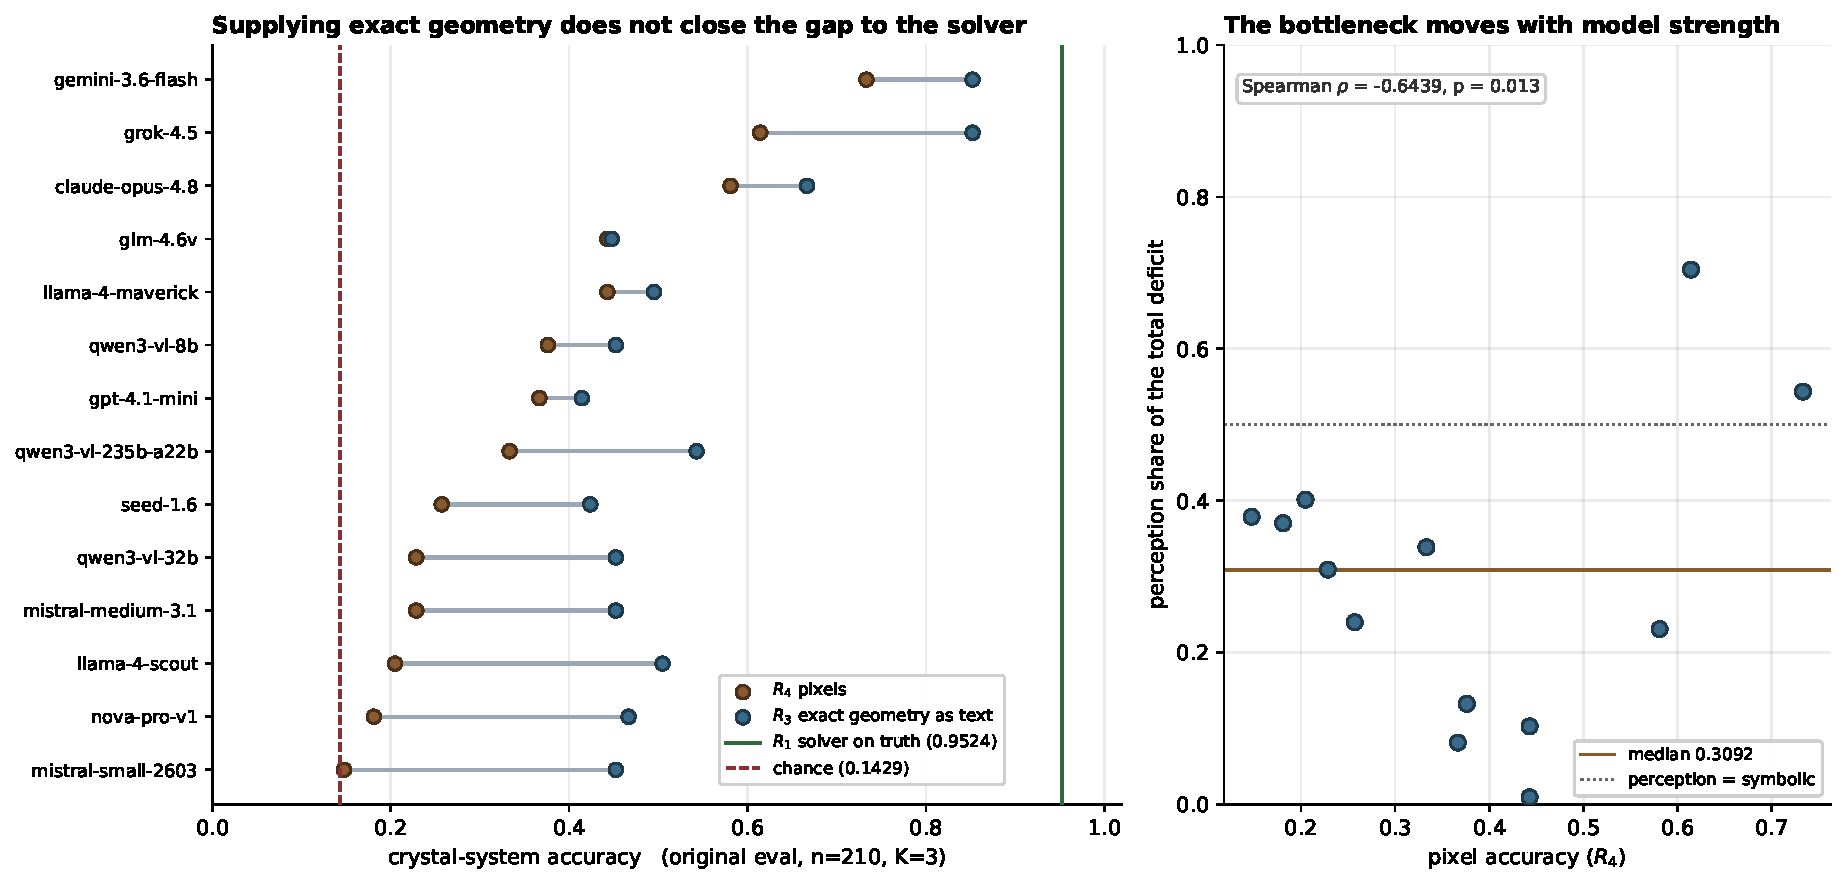
\includegraphics[width=0.8\linewidth]{figures/ladder.pdf}
\caption{Left: attribution ladder, original evaluation sample ($n=210$); rungs as in
Definition~\ref{def:ladder}, $R_2$ omitted (unscored under its pre-registered gate). Right: label ladder
across four label granularities for the model-free arms; the oracle (top curve) is flat, the cell-metric
baseline is not.}
\label{fig:ladder}
\end{figure}
